\documentclass[]{book}
%\usepackage{standalone} %you could combine documents this way 
\usepackage{booktabs} % tables
\usepackage{graphicx} %allows .png\
%\usepackage{natbib} % I don't think we need this, just chapterbib
\usepackage{chapterbib}

  % Smaller margins, fix these later:
\addtolength{\oddsidemargin}{-0.75in}
\addtolength{\evensidemargin}{-1.25in}
\addtolength{\textwidth}{1.75in}%
%\addtolength{\topmargin}{-1in}
\addtolength{\textheight}{1.5in}

\begin{document}
%\section*{Cover page}
\noindent Authors: Matthew Eklund, Christopher Morrison, and Jaron Senecal\\
Affiliation: Rensselaer Polytechnic Institute \\
Last updated: \today


\section*{Disclaimer}
This document is for informative and educational purposes only and is incomplete.  
The views and opinions expressed in this book do not necessarily represent those of Rensselaer Polytechnic Institute. 
Additional information will be added throughout the year. Don't sue us, please.


\section*{Preface}
%Well, it's simple...
Teaching college students how to solve equations is easy to do. But teaching students how to design systems is more complex, mostly because it is less regimented. From our experience as graduate students in nuclear engineering we feel that the process of designing reactors has not been adequately covered by the existing curriculum. Perhaps this is due to the fact that reactor designs seem limited to PWRs and new construction is quite rare. Our hope is that this book will help prepare young engineers to design the reactors of tomorrow. (Our hope is that we are among those engineers). Furthermore, all existing nuclear reactors were designed about fifty years ago, so our goal is to learn from those who were there when it happened. Perhaps this book can be used as the basis for a course in reactor design.

\begingroup
\let\cleardoublepage\clearpage
\tableofcontents
\endgroup

\chapter{Starting from a Clean Slate}

\section{Initial Design}
It all starts with a mission, a set of goals that must be accomplished. There are five types of missions: Commercial power, propulsion, science/medical, military, and political.
\begin{itemize}
  \item Commercial power. Missions typically state requirements on power rating, fuel loading cycle, and operability. Constraints are usually to satisfy regulatory requirements for safety. Design goals include anything from small modular reactors to breed and burn reactors to the familiar behemoth LWR. The idea is usually to maximize profits to the owner/operator.
  \item Propulsion. Nuclear fission provides a large supply of power in a very compact space. At various times the ability to continue almost indefinitely without refueling has been desired for marine, aeronautical, locomotive, and space propulsion. Thus the requirement is to minimize size and weight and provide power on demand.
  \item Science/medical. Small test reactors are desirable for producing irradiating targets. The goal may be to produce isotopes through neutron activation or fission or to test materials under neutron bombardment. Thus the goal is to provide neutron flux to a target. The product of these reactors is either data or isotopes. 
  \item Military. The power density of nuclear is desirable to the military because it eliminates the need for supply chains. (Sub)marine propulsion is the primary application, but there is also interest in land-based power. Cost becomes less of an issue for these applications and where power may be needed at a moment's notice.
  \item Political. Nuclear reactors may be commissioned as a demonstration of a country's technological capabilities. Due to the cost of R\&D and manufacturing, government leaders are often involved in the nuclear industry. Political missions may fulfill long term needs that could not be supported by commercial entities.
\end{itemize}

Given the mission, a list of requirements must be generated. There will be constraints and quantities to be optimized. For example, the customer desires maximum thermal flux, but also expects a safe reactor. This list of requirements and reactor attributes will guide the reactor design process.

Several key attributes are desirable for almost every nuclear reactor
\begin{itemize}
  \item Safety. Nuclear engineers are ethically responsible for designing reactors that will not harm the public.
  \item Economics. Saving money is always good.
  \item Efficient fuel utilization. 
  \item Non-proliferation. This reactor should not be an avenue for your enemies to acquire materials for nuclear weapons or dirty bombs.
  \item
\end{itemize}
There are many attributes that may be desirable or required for a reactor. The mission will dictate which features are necessary, desirable, or unneeded.
\begin{itemize}
  \item Minimizes enrichment requirements
  \item Breeds fissile material from fertile isotopes
  \item Destroys stockpiled fissile materials
  \item Destroys transuranic waste
  \item Minimizes total fissile material in-core inventory
  \item Longer intervals between refueling
  \item On-line refueling
  \item Provides high temperature process heat
  \item Capable of changing power rapidly to follow load demands
  \item Low weight to enable mobility or efficient propulsion
  \item High flux (fast or thermal) on target
\end{itemize}

Nuclear reactor design is multi-disciplinary by nature. Neutronics design affects thermal-hydraulic design and vice versa. Structural and material analysis must also be included. <insert flow-chart graphic>. The coupled effects between disciplines confound the design process, thus design iteration is necessary.

First the design parameters must be selected for each discipline. Pitch and diameter of the fuel pins affects thermal-hydraulics, whereas enrichment is a parameter of the neutronics design. It is necessary to obtain an understanding of how these parameters effect the metrics of interest. 

\section{Homework Problems}
\begin{enumerate}
\item (a) For each of the following reactor missions list several requirements and/or desirable attributes that the reactor should have. (b) List a type of reactor that would and one that would not be suitable for this mission.\\
A reactor for utilizing limited fuel resources. A reactor that can transmute actinides. A reactor that is proliferation resistant. 

\end{enumerate}

\section{Cold Fusion}
Some things are too good to be true. Often when people design a new paper reactor they describe it as the savior of the industry. The truth is, every reactor has a downside. Even a reactor that is optimized for one mission will be inadequate for other missions. It is important to keep an open mind when designing new reactors. But it is also important to make decisions based on analysis of \emph{all} the pertinent considerations. By all means be a proponent of your reactor design, but understand that it will have limitations. 


%Chapter 2
\chapter{How Did We Get Here? The History of Nuclear Energy}
In the field of nuclear technology, change is difficult. Developing materials that can withstand high temperatures and intense radiation is a timely, laborious process. 
Proving new technologies and demonstrating extreme reliability of parts  in any foreseeable environment is costly.
Imagining and protecting against extremely low-probability events is even more difficult for new ideas with unknown failure modes.

All of these hurdles and more must be overcome in order implement new reactor designs. At the time of this writing, it seems that these hurdles are so large in the United States that the LWRs will be the only design ever built here.
Indeed, looking back on the history of nuclear power, no reactor design has ever successfully reached market that was not driven primarily by the government. In other words, the benefits of advanced reactor designs are not enough to warrant the monumental investment from industry that would be needed to develop new technology. This is greatly exacerbated by the decades-long research and development time frame.

\section{World War II}
Fission was discovered in December 1938. It's potential was immediately realized and the race to develop the ultimate bomb began. Uranium bombs require enrichment facilities, but plutonium bombs could be fueled by reprocessed fuel from a reactor. Thus the mission for the first reactors was anything that could produce plutonium. The key attributes were the use of natural uranium and quick production time. Safety was established by siting the reactor in an uninhabited area of Washington state and following good engineering practices. Graphite moderated, water cooled reactors were the clear choice because heavy water was too scarce.
%something about uranium metal being the easiest to work with.

Following the war plutonium production was still a key objective so further breeder reactors were built at Hanford. Heavy water reactors were constructed at the Savannah River Site in South Carolina. All of the energy produced from fission was simply dumped into rivers, rather than used for generating electricity.

%Verify, get sources
%In Europe, graphite reactors were also used for breeder plutonium for weapons. The necessary modifications were made to 
% http://www.world-nuclear.org/information-library/current-and-future-generation/outline-history-of-nuclear-energy.aspx

In 1951 the EBR-I reactor demonstrated that nuclear reactors could be used to generate electricity. %what was the main thrust behind building this reactor?
In 1954, Russia began operation of the first nuclear reactor that was connected to an electrical generator with a rating of 5MWe.
Similarly, without sufficient enrichment capabilities, the United Kingdom used natural uranium metal, gas-cooled, graphite moderated reactors. The first of these came on line in 1956.
France followed a similar path as the UK with graphite moderated, gas cooled reactors. 
Canada completely avoided the path to enrichment and utilized their heavy water capabilities to create reactors. 

\section{Naval Reactors}
In the 1950s Admiral Hyman Rickover oversaw the development of pressurized water reactors. In order to fit a reactor into a submarine, highly enriched fuel and light water were used. In 1954 the USS Nautilus was launched. Zirconium purification was developed to support the naval reactors program---previously zirconium was unsuitable due to Hafnium impurities. 

With the research and development covered by the naval reactors program, light water reactors were now feasible for use by electrical utilities. In 1957 the Shippingport 60MWe reactor began operation as the first commercial nuclear reactor in the United States. %world?

\section{Design Evolution}
From the starting point of light water reactors, technology steadily improved performance without any major design changes. Most of these developments involve enhancing fuel performance. 
Various alloying elements were added to zirconium to improve corrosion resistance. This was essential for increasing the amount of time the cladding could survive in the core. 
In 1977 when President Carter banned reprocessing of fuel, reaching higher burnup became the key goal for fuel management. Until that point it had been understood by the industry that fuel would be reprocessed by the Atomic Energy Commission.

Controlling the grain size of sintered UO$_2$ allows for mitigating swelling and better retention of fission products. Creating a dished shape allows the pellets to accommodate thermal expansion and reduce stress on the cladding.  

% burnable absorbers
% chemical shim
% mention BWRs

\section{Growth of Safety Requirements}
From the very beginning, safety has been integral to the development of nuclear reactors. At the Chicago pile, Fermi stationed a Super-Critical Reactor Ax Man to drop boron into the reactor if anything should go wrong.
The plutonium production reactors were sited at Hanford to minimize the impact of a catastrophic failure.
Admiral Rickover demanded that those designing the submarines took as much care as if their sons were aboard the ships.

As an extra precaution, the Shippingport Reactor was constructed with a containment building in case of a reactor meltdown or malfunction. All of the subsequent reactors followed suit. 
Initial safety considerations followed the idea of the maximum credible accident. Initially this was a reactivity insertion. Commercial designs prevented withdrawing control rods too rapidly, so the next scenario to worry about was a Loss Of Coolant Accident (LOCA).
% http://users.owt.com/smsrpm/nksafe/sixties.html
After 1966, the Emergency Core Cooling System (ECCS) began to be viewed as necessary in order to prevent disastrous consequences of a LOCA.  ``it has certainly obtained the bulk of the resources expended in nuclear reactor safety research.''\cite{Safety_website}

In 1975 the Nuclear Regulatory Commission (the successor of the Atomic Energy Commission) published the Reactor Safety Study (WASH-1400). This report used Probabilistic Risk Assessment to estimate the risk that nuclear reactors pose to public health. The report showed that human error and small-break LOCAs were larger concerns than the maximum credible accidents that had been previously fixated on.

The 1979 accident at Three Mile Island unit 2 served as a wake-up call to the nuclear industry that serious accidents could occur. The importance of a safety culture became apparent. Human error finally became a major focus of safety. On the engineering side, better instrumentation and presentation in the control room were now clearly necessary

In the 1990s passive hydrogen recombiners were recommended as a retrofit.

\section{Other Reactor Designs}
Up to this point in the chapter only a few reactor types have been discussed. This is because nuclear technology has been inextricably linked to government research and development for military use. 
Graphite reactors cooled with either water or gas stemmed from plutonium production efforts as did heavy water reactors. %It should be noted that the Canadian government has foresworn enrichment of uranium and demonstrates no desire to produce plutonium for weapons.
Light water reactors grew out of naval propulsion programs. 

Given that the goals of commercial power plants differ from the military goals that the reactor designs grew out of, it is unlikely that these designs are optimal for power production. Furthermore, the perspective taken on issues of safety has significantly changed in the 50 years since the reactors began operation. 

To be fair, many reactor designs have been created and prototyped. Gas-cooled reactors, sodium-cooled fast reactors, organic-moderated reactors, molten-salt reactors, lead(-bismuth)-cooled reactors have all been operated. But they have all been discontinued because of various setbacks and challenges. Could it be that given a government R\&D push like LWRs experienced, that these advanced reactor designs would out-perform the current standard?

Perhaps the additional impetus will come from shortages of U-235. SFRs have received considerable attention throughout the years because they can accomplish a mission that thermal reactors cannot: breeding their own fuel.
But that goal has become less important as uranium ore deposits continue to be discovered.


%%%%%%%%%%%%%%%%%%%%%%%%%%

\begingroup
\let\cleardoublepage\clearpage

\bibliographystyle{ieeetr}
\bibliography{bib2}

\endgroup

\chapter{How to Begin}
This part might go in Chapter 1???

\section{Design Progression}
While it may be tempting to attack a design problem with all of the computational tools at your disposal, that may not be the best approach. Informed decisions at the beginning of the project reduce the amount of work that you and your computer will have to do. 
In general, low-fidelity methods or formulations are entirely satisfactory at the start. Simple calculations also tend to provide understanding and intuition that will be useful as the design process continues.

As the design matures, so should the tools being used. Think of computer codes as sieves. Low-fidelity codes will filter out designs that obviously won't work and more sophisticated tools may be needed to decide between closely competing design alternatives.

That being said, the ultimate goal is to reduce the time needed to generate a satisfactory design. There is no reason to spend more time on a less accurate method. For example, spending an hour to calculate the four-factor formula by hand with analytical methods is not as wise as waiting 15 minutes for the results from a Monte Carlo simulation. So the rough-cut tools you use should also be fast and easy to use.

While it is easier to describe a linear design process, that is usually not how it works in practice. Initially there will likely be several candidate designs which should be investigated in parallel. The number of competing designs will decrease as time goes on. 
Furthermore, design textbooks generally present the design process as a chronological journey through a serious of tasks. But this is not accurate, because design is an iterative process. So then the flow charts are given arrows for every point to every preceding point. 
With such a tangled picture in mind, we wish to emphasize from the outset that the design process will involve regular backtracking, especially since ideas are not generated only during brainstorming sessions.
The important thing is keep moving and maintain a willingness to backtrack, modify, and change your design. Trying to design an optimal reactor from the outset will certainly lead to slow going. So do your best to stay out of rabbit holes at the beginning and leave the details for later.

Insert a figure: flow chart or reactor categorization.

\section{Initial Decisions}
Some decisions can be made immediately based on engineering knowledge and an understanding of the design goals. Two of the most generic questions are What enrichment is acceptable? and What energy spectrum should the reactor have? The constraint of using natural uranium will quickly suggest a thermal reactor with only a few options for moderators. The desire to breed plutonium will dictate a high-neutron energy spectrum. 

After the obvious choices have been made, but without accidentally eliminating any viable choices, there are a few fundamental decisions to make. The choice of moderator (if needed), coolant, fuel isotope, and chemical fuel form are the fundamental features around which the reactor will be designed. These decisions do not require any computer simulations if the correct figures of merit are identified and used. 

Often selection is not straightforward because the materials are better at some things and worse in other respects. In cases like these, the decision is which set of issues you want to deal with.
The way each issue is weighted will influence the decision. For example, if low R\&D requirements is a priority, UO$_2$ will be selected and the poor thermal conductivity will have to be dealt with. 
Dichotomies like this help explain why there remains such a diversity of opinions and research efforts.
In other words, there may be more than one acceptable answer, but it is important to explain why the selection was made.

% Chris will probably want to expand this part quite a bit

\subsection{Coolant Selection}
Nuclear engineers often think of neutronic design as the critical (pun intended) part of the reactor system. However, neutron transport is actually a smaller part of the design than one would think.
In any reactor that produces power, cooling is essential. When the goal is producing electricity, managing the working fluid is the key to reliability and efficiency. Thus we begin with a discussion of coolants.

The first question is, Is this a thermal spectrum reactor? If the answer is no, many low-Z coolants are automatically eliminated from consideration.
Next, the desired operating temperatures need to be assigned ballpark numbers. This is determined by estimating the capabilities of heat exchangers, turbo-machinery, and structural and piping materials. You can prescribe these limits later if necessary, remember design is an iterative process. 

The following coolant properties are desirable for any reactor. \emph{High heat capacity}. This allows the coolant to absorb more energy per change in temperature. \emph{Non-corrosive}. Whatever the coolant contacts, or has the potential to contact, it should be compatible with. If the coolant corrodes the cladding, it will limit the fuel cycle length and sabotage the fuel utilization. \emph{Radiation stability} The coolant in the core will experience high radiation fields and radiolysis and neutron activation will occur. The coolant should be selected so that these phenomena are minimized. \emph{Low cross section} Neutrons absorbed in the coolant or coolant impurities will diminish the performance of the reactor.%\cite{Hausner}

%water
% liquid metal
% gas
% salts
% other

\subsubsection{Comparison of Liquid and Gaseous Coolants}
The phase of the coolant is an important consideration. Both liquid and gaseous coolants have their advantages and disadvantages.
If gaseous coolant is chosen, the chemically inert noble gases become attractive options.

\begin{table}[!ht]
\begin{tabular}{c|c|c|c}
  Qualtiy & Liquid & Two-Phase & Gaseous \\
  \hline
  Heat Capacity & High & High & Low \\
  Phase Change & Limiting condition & Desirable & Not an issue \\
  Heat Transfer Coefficient & High & Very high & Low \\
  Natural Circulation & Good & Very good & Poor \\
  Pumping Power & Low/good & Low/good & High/bad\\
  Neutron Absorption & High & Less & Low\\
  Direct Cycle & No & Yes, Rankine & Yes, Brayton\\
  Low Pressure & Maybe & No & No\\
  %
  \hline
\end{tabular}
\caption{Phase of coolant}
\end{table}

%\subsubsection{Comparison of Molten Salts and Liquid Metals}
%\subsubsection{Comparison of Moderating Coolants}
% or:
%\subsubsection{Comparison of Liquid Coolants}


\subsection{Moderator Selection}
For thermal reactors, a low-Z element is needed to slow down the fission neutrons to low energy levels where fission is more likely to occur. It must also do this without absorbing too many neutrons. Hydrogen is an obvious choice because of its ability to stop a neutron completely with only one scattering interaction and its low mean free path. Deuterium comes to mind next because it absorbs neutrons 1000 times less. Graphite is a desirable moderator because it can withstand extremely high temperatures.
%reproduce Duderstadt discussion and table

% \subsection{Figures of Merit}

\subsection{Fuel Selection}
The requirements of nuclear fuel are very demanding due to the environment it must withstand. Hausner %\cite{Hausner}
lists the following requirements for nuclear fuel
\begin{itemize}
\item[1.] It must be able to tolerant radiation damage
\item[2.] It must not corrode upon contact with the cladding or coolant.
\item[3.] It or its impurities must not absorb too many neutrons
\item[4a.] It must be able to withstand the temperature gradient caused by the heat it generates
\item[4b.] It should have high thermal conductivity (or appropriate dimensions) in order to transmit its heat to the coolant
\item[5.] It must be able to withstand the thermal cycles that it will experience during operation
\item[6.] It must be able to withstand the mechanical loads placed upon it
\item[7.] It must be inexpensive
\item[8.] It should lend itself to the fuel cycle in which it will be used, e.g. easy to reprocess
\end{itemize} 

Also it is generally preferable to have a high density in order to ease requirements for enrichment.

\subsection{Cladding Selection}
Material selection for cladding is important because it is the first line of defense for retaining radioactive material.
Even for reactor designs with no cladding, e.g. a molten salt-fueled reactor, it is necessary to select compatible and durable materials to contain the nuclear material and working fluid.
Selecting reliable cladding and piping materials allows the reactor to run smoothly with fewer interruptions. The primary requirement is for the cladding to be chemically compatible with both the fuel and the coolant. Superior corrosion performance is the foremost concern.

The cladding material must also be capable of enduring an extreme environment of neutron, gamma, and fission product irradiation and high temperatures. It must also maintain its strength and ductility while absorbing as few as possible neutrons. 
After all this, it would be preferable if the material was cheap and easy to manufacture.

\section{Geometric Specification}
After these have been determined, the basic core geometry comes next. Fuel pins increase centerline temperatures, but minimize the amount of cladding required, thus the neutronics expert prefers this option. The heat transfer expert prefers a design that tends towards a plate with more surface area per volume. 
%discuss other options: molten fuel, dispersions, particles
At this point an optimized design is unlikely and even unneeded. More likely each analysis will provide the limits of a feasible design space. 







\chapter*{Material Properties}
This appendix of material properties should be useful for initial comparison studies. For precise values several resources are recommend in a later section.


\begin{figure}[htbp]
  \centering
  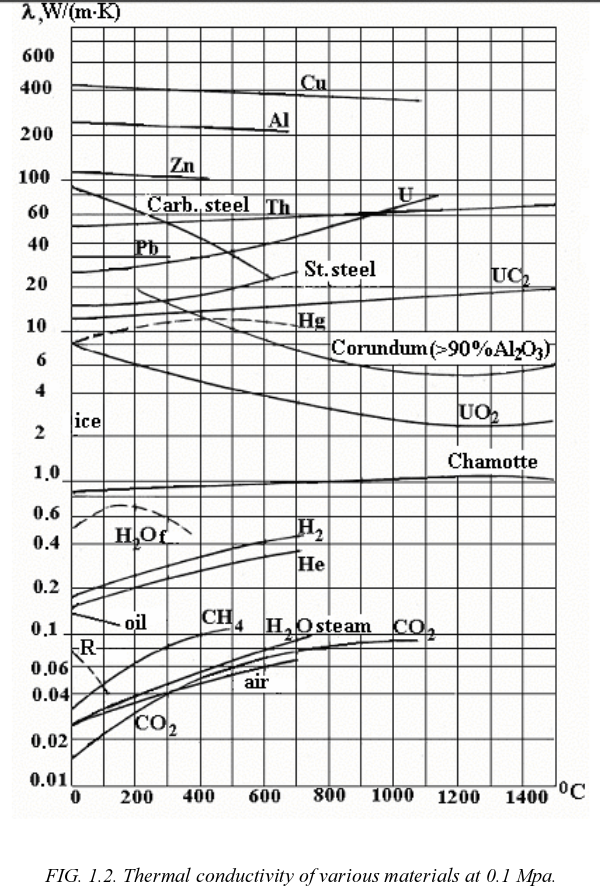
\includegraphics[width=4in]{graphics/thermal-k.png}  
  %\caption{Thermal conductivities}  
\end{figure}



\begin{table}
  \centering
  \caption{Basic Thermal Properties\cite{IAEA_1}}
  \begin{tabular}{lcccc}
    \toprule  
    Material & Conductivity & Density & Melting Point & Thermal Expansion\\ 
    %Heat Capacity,K/W/g
             & W/mK &    g/cm$^3$     &   $^{\circ}$C  &  1E6/$^{\circ}$C \\
    \midrule    
    UO$_2$ & 2.79 & 10.963 & 2800 & 9.8\\
    UN     & 20.9 & 14.42  & 2850 & 7.5\\
    UC     & 23   & 13.63  & 2365 & 10.5\\
    U metal & 31.2 & 19.1  & 1130 & 13.9\\
    U-20Pu-10Zr & 16 & 15.67 & 1155 &17\\
    U$_3$Si$_2$ & 22 & 12.2  & 1700 &16.1 \\
    \bottomrule
  \end{tabular}

\end{table}


A good resource has been provided by the IAEA\cite{IAEA_1}.


%%%%%%%%%%%%%%%%%%%%%%%%%%%%%%
\begingroup
\let\cleardoublepage\clearpage


\bibliographystyle{ieeetr}
\bibliography{matbib}

\endgroup


\end{document}